\documentclass[dvipsnames,mathserif]{beamer}
\setbeamertemplate{footline}[frame number]
\setbeamercolor{footline}{fg=black}
\setbeamerfont{footline}{series=\bfseries}
\usepackage{tikz}
\usepackage{xcolor}
\usepackage{graphicx, setspace, appendix, mathrsfs, amsmath, amsfonts,caption, mathtools}
\usepackage[english]{babel}
%\usetheme{Frankfurt}%1
\usetheme{Darmstadt}%1

% for RTL liste
\makeatletter
\newcommand{\RTListe}{\raggedleft\rightskip\leftm}
\newcommand{\leftm}{\@totalleftmargin}
\makeatother

% RTL frame title
\setbeamertemplate{frametitle}
{\vspace*{-1mm}
  \nointerlineskip
    \begin{beamercolorbox}[sep=0.3cm,ht=2.2em,wd=\paperwidth]{frametitle}
        \vbox{}\vskip-2ex%
        \strut\hskip1ex\insertframetitle\strut
        \vskip-0.8ex%
    \end{beamercolorbox}
}
% align subsection in toc
\makeatletter
\setbeamertemplate{subsection in toc}
{\leavevmode\rightskip=5ex%
  \llap{\raise0.1ex\beamer@usesphere{subsection number projected}{bigsphere}\kern1ex}%
  \inserttocsubsection\par%
}
\makeatother

% RTL triangle for itemize
\setbeamertemplate{itemize item}{\scriptsize\raise1.25pt\hbox{\donotcoloroutermaths$\blacktriangleleft$}} 

%\setbeamertemplate{itemize item}{\rule{4pt}{4pt}}

\defbeamertemplate{enumerate item}{square2}
{\LR{
    %
    \hbox{%
    \usebeamerfont*{item projected}%
    \usebeamercolor[bg]{item projected}%
    \vrule width2.25ex height1.85ex depth.4ex%
    \hskip-2.25ex%
    \hbox to2.25ex{%
      \hfil%
      {\color{fg}\insertenumlabel}%
      \hfil}%
  }%
}}

\setbeamertemplate{enumerate item}[square2]
\setbeamertemplate{navigation symbols}{}


\titlegraphic { 
\begin{tikzpicture}[overlay,remember picture, opacity=0.1,]
\node[] at (0, 2.9){
};\end{tikzpicture}}
\setbeamertemplate{caption}[numbered]
\begin{document}

\rightskip\rightmargin
\title{The role of information acquisition in matching markets: China's college admission mechanisms}
\author{Yao Luo}


\institute{Boston College}
\footnotesize{\date{\today }


\begin{frame}
\maketitle
\end{frame}


%\footnotesize \tableofcontents
%
\section{Motivation}
\begin{frame}{Motivation}
Theoretical results tell us:
\vspace{0.5cm}
    \begin{itemize}
        \item Full information? Costly information acquisition to discover preferences.(Corcoran et al. 2018, Dynarski et al. 2020, Grenet et al. 2019)\\
        \item Market designers should pay attention to the acquisition and flow of information.\\
        \item Finding regret-free stable matching $\Leftrightarrow$ finding market-clearing cutoffs.(Azevedo and Loshno. 2016, Immorlica et al. 2020)\\
        \item Information deadlocks. Market-clearing cutoffs $\rightarrow$ budget set $\rightarrow$ preference formation $\rightarrow$ determine cutoffs
    \end{itemize}
\end{frame}

\begin{frame}{Motivation}
Real mechanism implementations:
\vspace{0.5cm}
    \begin{itemize}
        \item Achieve approximately regret-free stable outcomes by providing external historical data with respect to perturbed capacities: Australia\\
        \item In 2023 Australia has 62,846 applicants, while China has 12,910,000 applicants. \\
        \item Parallel admission mechanism (PA) - Direct serial dictatorship (DirSD) with length restriction of the rank-ordered list (ROL)\\
        \item Inner Mongolia dynamic admission mechanism (IM) - Sequential serial dictatorship (SeqSD) + sequential moves by groups instead of individuals + time constraints\\
        \item In 2025 Inner Mongolia will give up IM and use PA. IM began in 2007. 
    \end{itemize}
\end{frame}

\begin{frame}{Motivation}
Why switch from IM to PA?
\vspace{0.5cm}
    \begin{itemize}
        \item Both PA and IM provides historical cutoff scores, but IM offers additional information regarding matching outcomes. Counterintuitive.\\
        \vspace{0.2cm}
        \item Theoretically and experimentally, SeqSD leads to higher student welfare than DirSD. (Hakimov et all. 2023)
    \end{itemize}
\end{frame}
\begin{frame}{Motivation}
Real life implementation of SeqSD: groups + time constraints
\begin{figure}[h!]
\centering
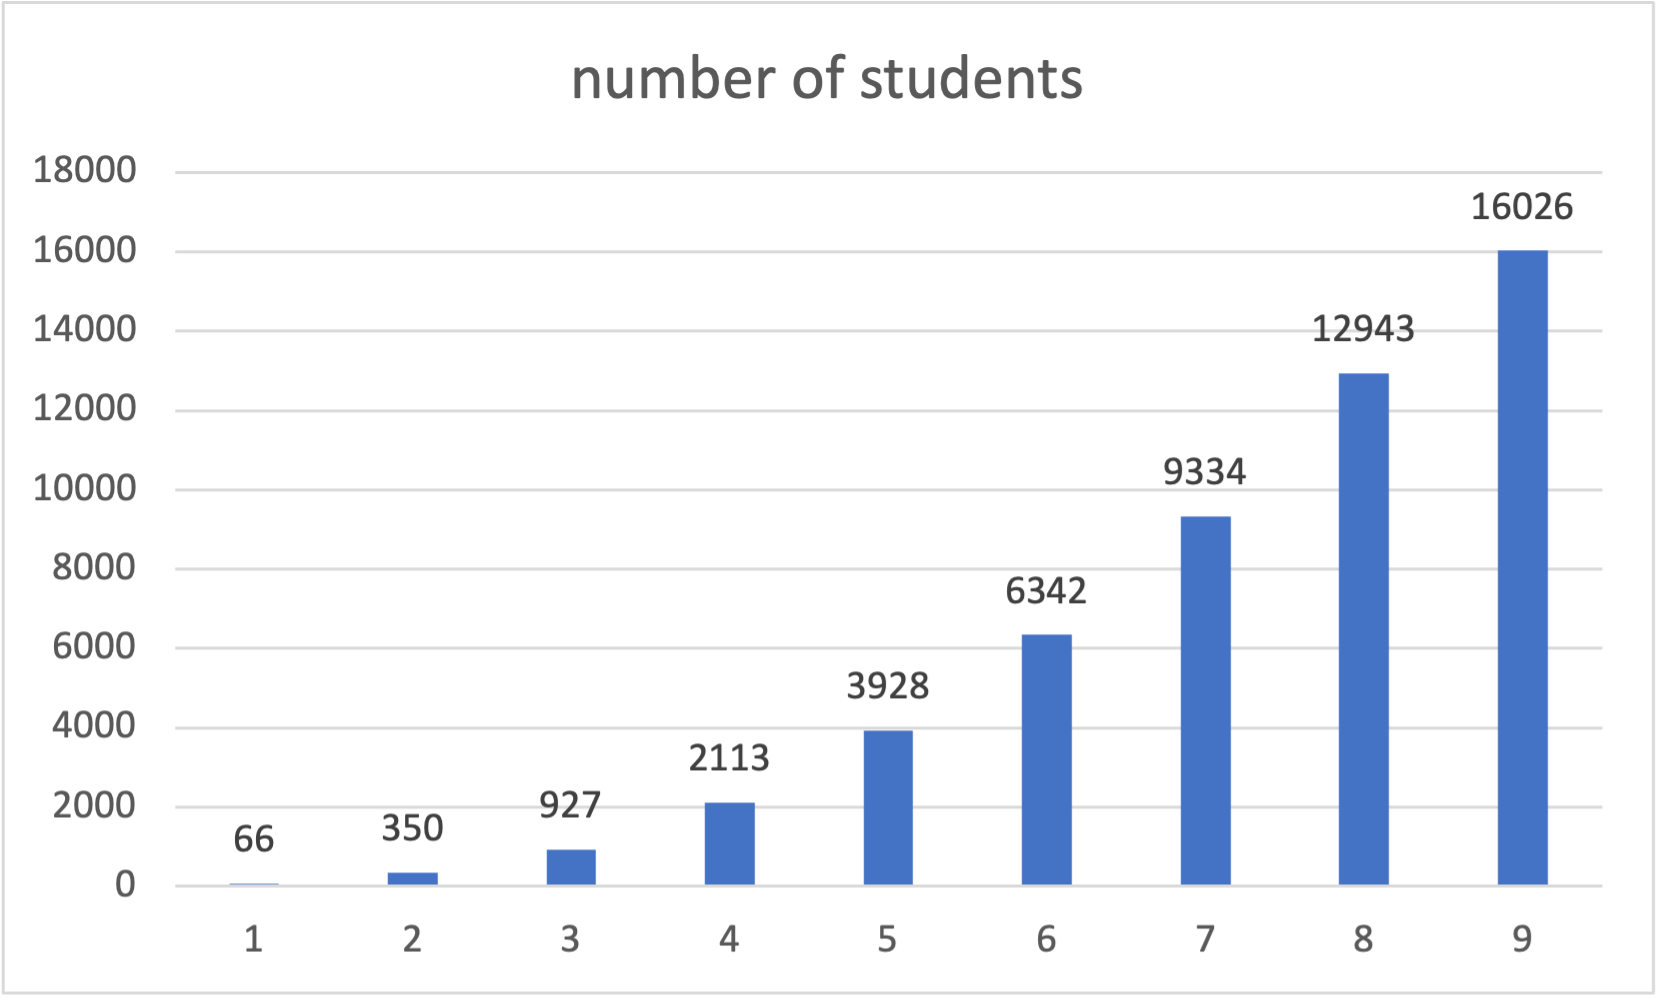
\includegraphics[width=0.8\textwidth]{1.png}
\end{figure}
\end{frame}




\section{Research question}
\begin{frame}{Research question}
Does PA result in higher student welfare than IM? If so why?
\vspace{0.5cm}
    \begin{itemize}
    	\item The time constraints in IM make the price discovery process too costly? 
        \vspace{0.2cm}
        \item Information communication in IM is not effective? 
        \vspace{0.2cm}
        \item The additional information is too noisy? 
        \vspace{0.2cm}
        \item Maybe IM is actually better than PA and the policy change is purely of political intention. 
        \vspace{0.2cm}
        \item Are there better ways to communicate information to students in IM?
    \end{itemize}
\end{frame}

\section{Contribution}
\begin{frame}{Contribution}
    \begin{itemize}
        \item Provide empirical and experimental comparisions of real-life implementation of DirSD (PA) and SeqSD (IM) mechanisms.
        \vspace{0.2cm}
        \item Shed light on the importance of information flows in market design and validate costly endogenous information acquisition.
        \vspace{0.2cm}
        \item Gong and Liang (2023) shows experimentally IM mechanism achieves similar stability as DA mechanism and similar efficiency as Bostom mechanism. Incomplete information. Low correlation of preferences.
        \vspace{0.2cm}
        \item Chen and Kesten (2019) shows experimentally DA mechanism is better than PA in terms of stability, but the setup assumes complete information.   
    \end{itemize}
\end{frame}


\section{Empirical strategy}
\begin{frame}{Empirical strategy}
	\begin{itemize}
		\item Data: students' gender, ethnicity, exam score, rank and admission result.
        \item \[y_i = \alpha_0 + \alpha_1 X_i + \beta Y_{2025} + \varepsilon_i\]
        $y_i$: college prestige index. Calculated by dividing the rank of the college (determined by cutoff scores of year 2022 and 2023) by the total number of colleges.\\
        $X_i$: students' gender, ethnicity, rank by exam scores being normalized to be within (0,1).\\
        \item Implicitly assumes higher-ranked students prefer more prestigious colleges. Only care about big names without considering majors. \\
        \item Spearman's rank correlation coefficient.
        \[\rho = 1 -  \frac{6\Sigma_{i}^{N}d_i^2}{n(n^2-1)}\]
        
    \end{itemize}
\end{frame}

\section{Experiment design}
\begin{frame}{Experiment design}
General setup:
\vspace{0.5cm}
    \begin{itemize}
        \item Exam scores are randomly and independently drawn from the IM empirical distribution between 0 and 100.
        \item Students know their exam scores, ranks, each university's quotas and historical cutoffs. 
        \item 30 students competing for 15 seats in 10 colleges. Admission rate is 50\%.
        \item Preferences are private knowledge. Students need to pay search costs to acquire information about their own preferences.\\
    \end{itemize}

\end{frame}

\begin{frame}{Experiment design}
Environments:
\vspace{0.5cm}
    \begin{itemize}
        \item Dimension 1: The degree of correlation of preferences among students.\\
        \item Dimension 2: The cost of information acquisiton.
    \end{itemize}
\end{frame}

\begin{frame}{Experiment design}
Predictions:
\vspace{0.5cm}
    \begin{itemize}
        \item Hypothesis 1: Lower-ranked students gain more from IM compared to PA.\\
        \item Hypothesis 2: Lowest-ranked student in each group is worse off than under PA.\\ 
        \item Hypothesis 3: IM has a higher probability of being unmatched.\\
        \item Hypothesis 4: Given an extended time constraint, students may oversearch.\\
        \item Hypothesis 5: Smaller group size produces better matching outcomes.\\
        \item Hypothesis 6: Increasing the ROL in PA improves the matching outcomes.
    \end{itemize}
\end{frame}

\section{Empirical distribution}
\begin{frame}{Empirical distribution}
    \begin{figure}[h!]
    \centering
    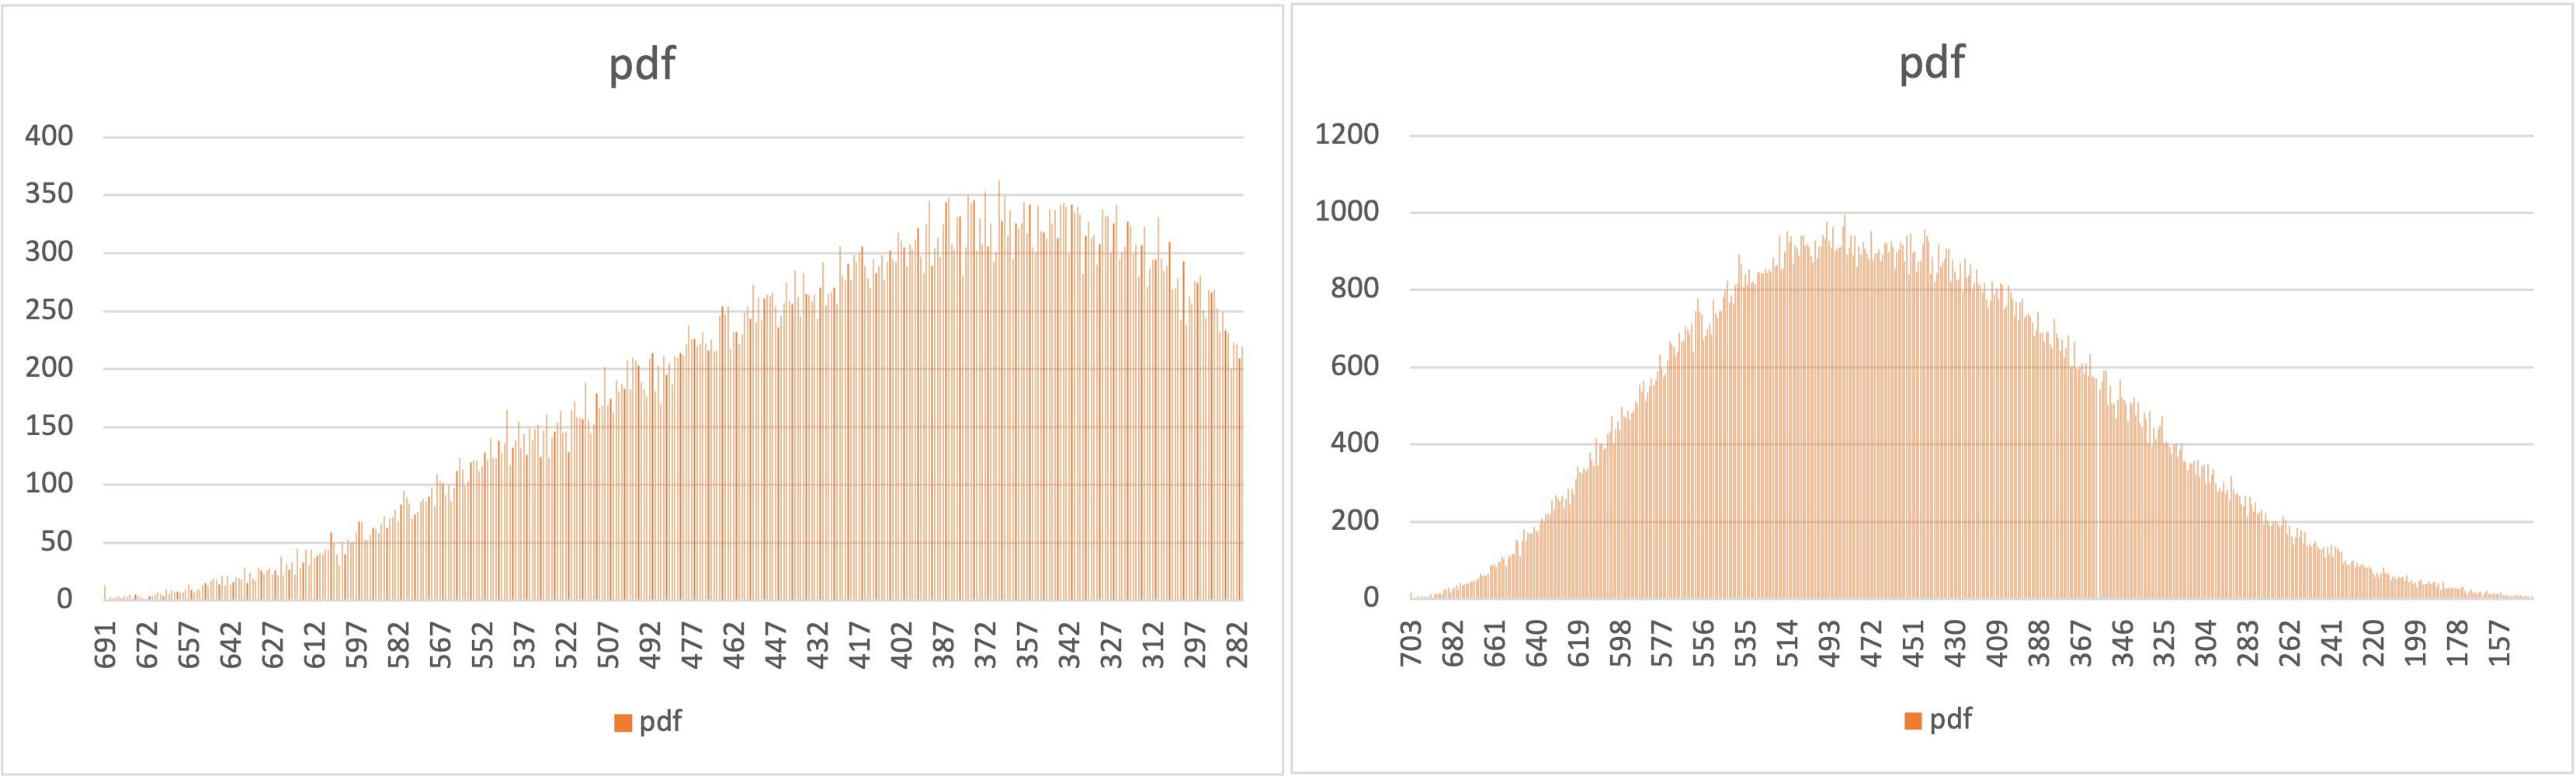
\includegraphics[width=\textwidth]{pdf.png}
    \end{figure}
\end{frame}

\end{document}